% Created by tikzDevice version 0.6.2-92-0ad2792 on 2013-01-08 03:49:56
% !TEX encoding = UTF-8 Unicode
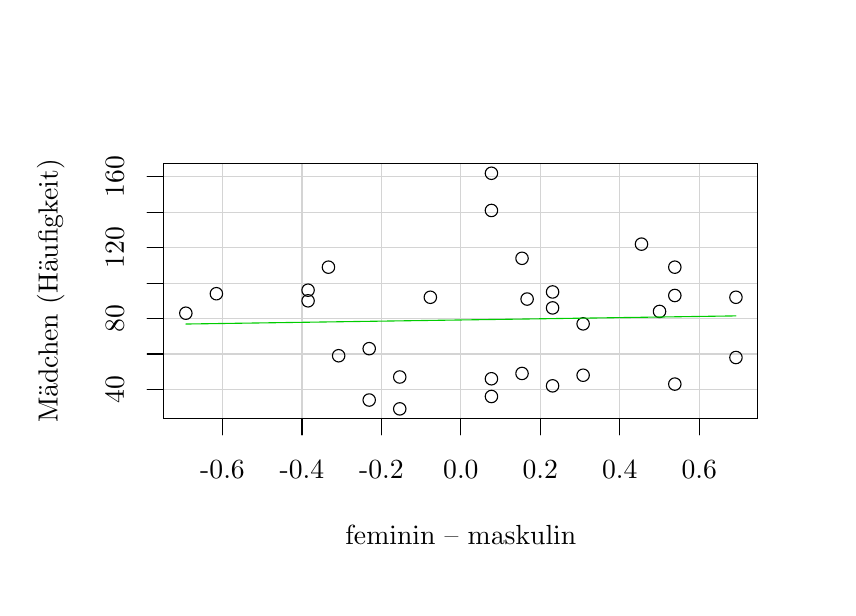
\begin{tikzpicture}[x=1pt,y=1pt]
\definecolor[named]{fillColor}{rgb}{1.00,1.00,1.00}
\path[use as bounding box,fill=fillColor,fill opacity=0.00] (0,0) rectangle (289.08,202.36);
\begin{scope}
\path[clip] (  0.00,  0.00) rectangle (289.08,202.36);
\definecolor[named]{drawColor}{rgb}{0.00,0.00,0.00}

\path[draw=drawColor,line width= 0.4pt,line join=round,line cap=round] ( 70.40, 61.20) -- (242.68, 61.20);

\path[draw=drawColor,line width= 0.4pt,line join=round,line cap=round] ( 70.40, 61.20) -- ( 70.40, 55.20);

\path[draw=drawColor,line width= 0.4pt,line join=round,line cap=round] ( 99.12, 61.20) -- ( 99.12, 55.20);

\path[draw=drawColor,line width= 0.4pt,line join=round,line cap=round] (127.83, 61.20) -- (127.83, 55.20);

\path[draw=drawColor,line width= 0.4pt,line join=round,line cap=round] (156.54, 61.20) -- (156.54, 55.20);

\path[draw=drawColor,line width= 0.4pt,line join=round,line cap=round] (185.25, 61.20) -- (185.25, 55.20);

\path[draw=drawColor,line width= 0.4pt,line join=round,line cap=round] (213.96, 61.20) -- (213.96, 55.20);

\path[draw=drawColor,line width= 0.4pt,line join=round,line cap=round] (242.68, 61.20) -- (242.68, 55.20);

\node[text=drawColor,anchor=base,inner sep=0pt, outer sep=0pt, scale=  1.00] at ( 70.40, 39.60) {-0.6};

\node[text=drawColor,anchor=base,inner sep=0pt, outer sep=0pt, scale=  1.00] at ( 99.12, 39.60) {-0.4};

\node[text=drawColor,anchor=base,inner sep=0pt, outer sep=0pt, scale=  1.00] at (127.83, 39.60) {-0.2};

\node[text=drawColor,anchor=base,inner sep=0pt, outer sep=0pt, scale=  1.00] at (156.54, 39.60) {0.0};

\node[text=drawColor,anchor=base,inner sep=0pt, outer sep=0pt, scale=  1.00] at (185.25, 39.60) {0.2};

\node[text=drawColor,anchor=base,inner sep=0pt, outer sep=0pt, scale=  1.00] at (213.96, 39.60) {0.4};

\node[text=drawColor,anchor=base,inner sep=0pt, outer sep=0pt, scale=  1.00] at (242.68, 39.60) {0.6};

\path[draw=drawColor,line width= 0.4pt,line join=round,line cap=round] ( 49.20, 71.65) -- ( 49.20,148.47);

\path[draw=drawColor,line width= 0.4pt,line join=round,line cap=round] ( 49.20, 71.65) -- ( 43.20, 71.65);

\path[draw=drawColor,line width= 0.4pt,line join=round,line cap=round] ( 49.20, 84.45) -- ( 43.20, 84.45);

\path[draw=drawColor,line width= 0.4pt,line join=round,line cap=round] ( 49.20, 97.26) -- ( 43.20, 97.26);

\path[draw=drawColor,line width= 0.4pt,line join=round,line cap=round] ( 49.20,110.06) -- ( 43.20,110.06);

\path[draw=drawColor,line width= 0.4pt,line join=round,line cap=round] ( 49.20,122.86) -- ( 43.20,122.86);

\path[draw=drawColor,line width= 0.4pt,line join=round,line cap=round] ( 49.20,135.67) -- ( 43.20,135.67);

\path[draw=drawColor,line width= 0.4pt,line join=round,line cap=round] ( 49.20,148.47) -- ( 43.20,148.47);

\node[text=drawColor,rotate= 90.00,anchor=base,inner sep=0pt, outer sep=0pt, scale=  1.00] at ( 34.80, 71.65) {40};

\node[text=drawColor,rotate= 90.00,anchor=base,inner sep=0pt, outer sep=0pt, scale=  1.00] at ( 34.80, 97.26) {80};

\node[text=drawColor,rotate= 90.00,anchor=base,inner sep=0pt, outer sep=0pt, scale=  1.00] at ( 34.80,122.86) {120};

\node[text=drawColor,rotate= 90.00,anchor=base,inner sep=0pt, outer sep=0pt, scale=  1.00] at ( 34.80,148.47) {160};

\path[draw=drawColor,line width= 0.4pt,line join=round,line cap=round] ( 49.20, 61.20) --
	(263.88, 61.20) --
	(263.88,153.16) --
	( 49.20,153.16) --
	( 49.20, 61.20);
\end{scope}
\begin{scope}
\path[clip] (  0.00,  0.00) rectangle (289.08,202.36);
\definecolor[named]{drawColor}{rgb}{0.00,0.00,0.00}

\node[text=drawColor,anchor=base,inner sep=0pt, outer sep=0pt, scale=  1.00] at (156.54, 15.60) {feminin -- maskulin};

\node[text=drawColor,rotate= 90.00,anchor=base,inner sep=0pt, outer sep=0pt, scale=  1.00] at ( 10.80,107.18) {Mädchen (Häufigkeit)};
\end{scope}
\begin{scope}
\path[clip] ( 49.20, 61.20) rectangle (263.88,153.16);
\definecolor[named]{drawColor}{rgb}{0.83,0.83,0.83}

\path[draw=drawColor,line width= 0.4pt,line join=round,line cap=round] ( 70.40, 61.20) -- ( 70.40,153.16);

\path[draw=drawColor,line width= 0.4pt,line join=round,line cap=round] ( 99.12, 61.20) -- ( 99.12,153.16);

\path[draw=drawColor,line width= 0.4pt,line join=round,line cap=round] (127.83, 61.20) -- (127.83,153.16);

\path[draw=drawColor,line width= 0.4pt,line join=round,line cap=round] (156.54, 61.20) -- (156.54,153.16);

\path[draw=drawColor,line width= 0.4pt,line join=round,line cap=round] (185.25, 61.20) -- (185.25,153.16);

\path[draw=drawColor,line width= 0.4pt,line join=round,line cap=round] (213.96, 61.20) -- (213.96,153.16);

\path[draw=drawColor,line width= 0.4pt,line join=round,line cap=round] (242.68, 61.20) -- (242.68,153.16);

\path[draw=drawColor,line width= 0.4pt,line join=round,line cap=round] ( 49.20, 71.65) -- (263.88, 71.65);

\path[draw=drawColor,line width= 0.4pt,line join=round,line cap=round] ( 49.20, 84.45) -- (263.88, 84.45);

\path[draw=drawColor,line width= 0.4pt,line join=round,line cap=round] ( 49.20, 97.26) -- (263.88, 97.26);

\path[draw=drawColor,line width= 0.4pt,line join=round,line cap=round] ( 49.20,110.06) -- (263.88,110.06);

\path[draw=drawColor,line width= 0.4pt,line join=round,line cap=round] ( 49.20,122.86) -- (263.88,122.86);

\path[draw=drawColor,line width= 0.4pt,line join=round,line cap=round] ( 49.20,135.67) -- (263.88,135.67);

\path[draw=drawColor,line width= 0.4pt,line join=round,line cap=round] ( 49.20,148.47) -- (263.88,148.47);
\end{scope}
\begin{scope}
\path[clip] (  0.00,  0.00) rectangle (289.08,202.36);
\definecolor[named]{drawColor}{rgb}{0.00,0.00,0.00}

\path[draw=drawColor,line width= 0.4pt,line join=round,line cap=round] ( 49.20, 61.20) --
	(263.88, 61.20) --
	(263.88,153.16) --
	( 49.20,153.16) --
	( 49.20, 61.20);
\end{scope}
\begin{scope}
\path[clip] ( 49.20, 61.20) rectangle (263.88,153.16);
\definecolor[named]{drawColor}{rgb}{0.00,0.00,0.00}

\path[draw=drawColor,line width= 0.4pt,line join=round,line cap=round] (167.58, 75.49) circle (  2.25);

\path[draw=drawColor,line width= 0.4pt,line join=round,line cap=round] (134.45, 64.61) circle (  2.25);

\path[draw=drawColor,line width= 0.4pt,line join=round,line cap=round] (134.45, 76.13) circle (  2.25);

\path[draw=drawColor,line width= 0.4pt,line join=round,line cap=round] (178.63,119.02) circle (  2.25);

\path[draw=drawColor,line width= 0.4pt,line join=round,line cap=round] (178.63, 77.41) circle (  2.25);

\path[draw=drawColor,line width= 0.4pt,line join=round,line cap=round] (200.71, 76.77) circle (  2.25);

\path[draw=drawColor,line width= 0.4pt,line join=round,line cap=round] (228.32, 99.82) circle (  2.25);

\path[draw=drawColor,line width= 0.4pt,line join=round,line cap=round] (108.69,115.82) circle (  2.25);

\path[draw=drawColor,line width= 0.4pt,line join=round,line cap=round] (167.58,149.75) circle (  2.25);

\path[draw=drawColor,line width= 0.4pt,line join=round,line cap=round] ( 68.19,106.22) circle (  2.25);

\path[draw=drawColor,line width= 0.4pt,line join=round,line cap=round] (167.58,136.31) circle (  2.25);

\path[draw=drawColor,line width= 0.4pt,line join=round,line cap=round] (112.37, 83.81) circle (  2.25);

\path[draw=drawColor,line width= 0.4pt,line join=round,line cap=round] (200.71, 95.33) circle (  2.25);

\path[draw=drawColor,line width= 0.4pt,line join=round,line cap=round] (233.84,115.82) circle (  2.25);

\path[draw=drawColor,line width= 0.4pt,line join=round,line cap=round] (180.47,104.30) circle (  2.25);

\path[draw=drawColor,line width= 0.4pt,line join=round,line cap=round] (123.41, 67.81) circle (  2.25);

\path[draw=drawColor,line width= 0.4pt,line join=round,line cap=round] (167.58, 69.09) circle (  2.25);

\path[draw=drawColor,line width= 0.4pt,line join=round,line cap=round] (145.50,104.94) circle (  2.25);

\path[draw=drawColor,line width= 0.4pt,line join=round,line cap=round] (189.67, 72.93) circle (  2.25);

\path[draw=drawColor,line width= 0.4pt,line join=round,line cap=round] (101.32,107.50) circle (  2.25);

\path[draw=drawColor,line width= 0.4pt,line join=round,line cap=round] (255.93,104.94) circle (  2.25);

\path[draw=drawColor,line width= 0.4pt,line join=round,line cap=round] (101.32,103.66) circle (  2.25);

\path[draw=drawColor,line width= 0.4pt,line join=round,line cap=round] (233.84, 73.57) circle (  2.25);

\path[draw=drawColor,line width= 0.4pt,line join=round,line cap=round] ( 57.15, 99.18) circle (  2.25);

\path[draw=drawColor,line width= 0.4pt,line join=round,line cap=round] (189.67,106.86) circle (  2.25);

\path[draw=drawColor,line width= 0.4pt,line join=round,line cap=round] (233.84,105.58) circle (  2.25);

\path[draw=drawColor,line width= 0.4pt,line join=round,line cap=round] (189.67,101.10) circle (  2.25);

\path[draw=drawColor,line width= 0.4pt,line join=round,line cap=round] (255.93, 83.17) circle (  2.25);

\path[draw=drawColor,line width= 0.4pt,line join=round,line cap=round] (221.80,124.14) circle (  2.25);

\path[draw=drawColor,line width= 0.4pt,line join=round,line cap=round] (123.41, 86.37) circle (  2.25);
\definecolor[named]{drawColor}{rgb}{0.00,0.80,0.00}

\path[draw=drawColor,line width= 0.4pt,line join=round,line cap=round] ( 57.15, 95.27) --
	(255.93, 98.21);
\end{scope}
\end{tikzpicture}
